% Use only LaTeX2e, calling the article.cls class and 12-point type.

\documentclass[12pt]{article}

% Users of the {thebibliography} environment or BibTeX should use the
% scicite.sty package, downloadable from *Science* at
% www.sciencemag.org/about/authors/prep/TeX_help/ .
% This package should properly format in-text
% reference calls and reference-list numbers.

\usepackage{scicite}

% Use times if you have the font installed; otherwise, comment out the
% following line.

\usepackage{times}
\usepackage{pgfplots}
\usepackage{amsmath}

% The preamble here sets up a lot of new/revised commands and
% environments.  It's annoying, but please do *not* try to strip these
% out into a separate .sty file (which could lead to the loss of some
% information when we convert the file to other formats).  Instead, keep
% them in the preamble of your main LaTeX source file.


% The following parameters seem to provide a reasonable page setup.

\topmargin 0.0cm
\oddsidemargin 0.2cm
\textwidth 16cm 
\textheight 21cm
\footskip 1.0cm


%The next command sets up an environment for the abstract to your paper.

\newenvironment{sciabstract}{%
\begin{quote} \bf}
{\end{quote}}


% If your reference list includes text notes as well as references,
% include the following line; otherwise, comment it out.

\renewcommand\refname{References and Notes}

% The following lines set up an environment for the last note in the
% reference list, which commonly includes acknowledgments of funding,
% help, etc.  It's intended for users of BibTeX or the {thebibliography}
% environment.  Users who are hand-coding their references at the end
% using a list environment such as {enumerate} can simply add another
% item at the end, and it will be numbered automatically.

\newcounter{lastnote}
\newenvironment{scilastnote}{%
\setcounter{lastnote}{\value{enumiv}}%
\addtocounter{lastnote}{+1}%
\begin{list}%
{\arabic{lastnote}.}
{\setlength{\leftmargin}{.22in}}
{\setlength{\labelsep}{.5em}}}
{\end{list}}


% Include your paper's title here

\title{Is team gamer frustration justified? \\
	\large The effect of team size on the convergence of Elo-rating}


% Place the author information here.  Please hand-code the contact
% information and notecalls; do *not* use \footnote commands.  Let the
% author contact information appear immediately below the author names
% as shown.  We would also prefer that you don't change the type-size
% settings shown here.

\author
{Rik Dolfing, Michiel Marcus, Rik van Toor}

% Include the date command, but leave its argument blank.

\date{}



%%%%%%%%%%%%%%%%% END OF PREAMBLE %%%%%%%%%%%%%%%%



\begin{document} 

% Double-space the manuscript.

\baselineskip24pt

% Make the title.

\maketitle 



% Place your abstract within the special {sciabstract} environment.

\begin{sciabstract}
  A common exclamation amongst gamers is that they cannot climb to their alleged skill, due to the abilities, or rather inabilities of the team. Although it is easy to play the blame game, the bigger question is whether this is justified. Therefore this research studies the relation between team size and Elo convergence rate. Using Monte Carlo simulations, a positive linear relation was found, showing that team size affects the time it takes a player to converge to their true Elo rating. However, the results show that players eventually converge to their true skill, although this might take more games. Thus, failing to climb the ladder for a long time can only be explained by insufficient proficiency, and not the team.
\end{sciabstract}



% In setting up this template for *Science* papers, we've used both
% the \section* command and the \paragraph* command for topical
% divisions.  Which you use will of course depend on the type of paper
% you're writing.  Review Articles tend to have displayed headings, for
% which \section* is more appropriate; Research Articles, when they have
% formal topical divisions at all, tend to signal them with bold text
% that runs into the paragraph, for which \paragraph* is the right
% choice.  Either way, use the asterisk (*) modifier, as shown, to
% suppress numbering.
\clearpage
\section{Introduction}

In a competitive gaming environment, your rank represents how good you are relative to others. With team based games, people tend to say :  ``I do not belong at this skill rating.'' \cite{exampleclaim}. To find out whether these accusation are valid, this study answers the question: Does a player's rating always converge to their own skill level? In order to answer this question, this study focused on the influence of team size on the convergence of a player's rating.

This study used the Elo rating system. The Elo rating system \textit{Elo}\cite{elo} is a rating system that can be used to determine a player's relative skill. The system was originally created with \textit{Chess} in mind, which is a one-versus-one environment. However, gradually more and more implementations were found. Nowadays, a great number of video games make use of this system in some way, whether it is an unaltered version or a deeply adjusted one. 

There already exist rating systems designed to support team based ratings. Popular choices are Mark Glickman's \textit{Glicko} and \textit{Glicko2}\cite{glicko}, as well as Microsoft's \textit{TrueSkill}\texttrademark\cite{trueskill}, which was based on some of the core concepts of \textit{Glicko}. These are algorithms were tailored to support teams, whilst the traditional Elo system was not. However, instructions forced the use of the traditional Elo system. Therefore, this research extends the original Elo system and applies it to a variety of team sizes. \\

\section{Method}
To simulate the workings of this system, a program based on Monte Carlo simulations\cite{montecarlo} was written. The program used is described using a step-by-step plan with elaboration where necessary.

\subsection{Elo}

The Elo system describes a function to determine the chance that a player will beat another player.\\

\textbf{Definition 1.} Given players $A$ and $B$ with rating $R_A$ and $R_B$ respectively, the chance $E_A$ that player $A$ beats player $B$ equals\\
\[ E_A = \frac{1}{1 + 10^{\frac{R_{B}-R_{A}}{400}}} \]\\

Additionally, the Elo system describes a function to adjust a player’s Elo rating after a game.\\

\textbf{Definition 2.} Given chance $E_A$ that player $A$ beats player $B$, player $A$'s new Elo rating equals
\[R' = \begin{cases}
R + (1 - E_A ) \cdot K & if \; won \\ R - E_A \cdot K & if \; lost
\end{cases}\]
Where
\[ K = \begin{cases}
16 & R < 2000 \\ 12 & 2000 \leq R \leq 2200 \\ 10 & R > 2200 
\end{cases}\]

https://nl.wikipedia.org/wiki/Elo-rating


\subsection{Assumptions}
A player’s Elo Rating has converged if their Elo does not change significantly over a span of at least 5\% of the number of games played so far. This is checked by taking the standard deviation of the player's Elo rating over the most recent games with regard to the player’s true skill. If this deviation is lower than a certain constant $\alpha$, the Elo rating has converged. To get to the value of $\alpha$, the following calculation was used:
\[R' = R + (W - P) \cdot K\]
\[\Delta R = (W - P) \cdot K\]
Since $(W - P)$ ranges from $-1$ to $1$, the maximum value of $\Delta R$ equals the maximum value of $K$: $16$. The minimum value of $\Delta R$ equals $-16$. Since the player will lose approximately the same number of games as they win, since they play against players of the same skill level, their Elo will fluctuate their true skill $\pm \Delta R$. To be on the safe side, the value of $\alpha$ was set to $20$.\\
The Elo rating itself is clamped between 1200 and 2800, which means that a rating cannot go lower than 1200 nor higher than 2800. Every new player starts at 1500 Elo, whilst the team size can be any positive integer.
Because of the League of Legends based matchmaking, if a player's true skill exceeds the opponent's true skill by at least 100 points, the chance becomes 1 that this player wins.\\

\subsection{Matchmaking}

The proposed program uses the same matchmaking technique as the popular online game \textit{League of Legends} does.

\begin{quote}
``... it computes the average of the player ranking values for each team, and then uses these averages to match teams similarly to one-versus-one fights.''\cite{moba}
\end{quote}


\subsection{Evaluation function}
The members of both teams are subdivided into couples. This means that each player on a team is matched with one opponent. Each individual win earns a win chance of $\frac{1}{N}$ where $N$ represents the team size. 
For example, in a situation with teams of size 3, all members of team A and team B will be paired up.\\
\textbf{Example}
\begin{quote}
A\textsubscript{1} versus B\textsubscript{1}, A\textsubscript{2} versus B\textsubscript{2}, A\textsubscript{3} versus B\textsubscript{3}.
If A\textsubscript{1} beats B\textsubscript{1}, A\textsubscript{2} beats B\textsubscript{2}, but A\textsubscript{3} loses to B\textsubscript{3}, the values will be $\frac{1}{3}$, $\frac{1}{3}$ and $0$ respectively. Thus, the accumulated value of this round equals $\frac{2}{3}$.
\end{quote}

This accumulated value will be referred to as \textit{factor 1} in future reference. This is a factor that is prominent within Multiplayer Online Battle Arena games such as League of Legends\cite{moba}.The ability to outsmart or outplay an opponent in a 1 versus 1 setting can determine the outcome of an entire game. However, an equally important factor is the ability to play together. This is the core of most games involving teamwork. For that reason, the average of the true skill is taken for both teams. This average will be referred to as \textit{factor 2} in future reference.
Lastly, the average of \textit{factor 1} and \textit{factor 2} is inserted into the original Elo win chance function mentioned in the Introduction section.

\subsection{The program}
The program uses 4 main variables. These are the number of simulations($S$), a team size($N$), the evaluation function($e$)  and the maximum difference between players called the competence range($c$). There are two phases in the program: the \textit{initialisation phase} and the \textit{game phase}. In the \textit{initialisation phase}, a new player($p$) is created which is monitored by the program, with a random true skill level $t$  and a starting Elo of $1500$. Starting the game phase, $N - 1$ random allies($a$) are added to $p$’s team. N Random opponents($o$) are added to the other team. For all generated opponents and allies, the Elo rating is calculated by
\[Elo_p \pm RandomMax(0,c)\]
When each $a$ and $o$ have been determined, the evaluation function(section 3.3) calculates which team wins and what the new rating of $p$ will become. If $p$'s Elo stays within $Elo_p \pm 20$ for 5\% of the games played so far, the player's Elo rating has converged.

\section{Results}
Using the program described in the Methods section, the following data was generated.
For each team size, a sample size of $10000$ simulations was used. In order to identify the effect of team size, the simulations were run with different competence values. The confidence intervals have a probability of $0.95$.

\begin{table}[!htb]
	\centering
	\caption{Using competence range 50}
	\begin{tabular}{llll}
		\textbf{Team Size} & \textbf{Average} & \textbf{Standard Deviation} & \textbf{Confidence Interval} \\
		1                  & 193              & 11                          & 193 - 193                    \\
		2                  & 229              & 66                          & 228 - 230                    \\
		3                  & 280              & 126                         & 278 - 282                    \\
		4                  & 341              & 187                         & 337 - 345                    \\
		5                  & 404              & 245                         & 399 - 409                    \\
		6                  & 474              & 306                         & 468 - 480                    \\
		7                  & 537              & 365                         & 530 - 544                    \\
		8                  & 595              & 414                         & 587 - 603                    \\
		9                  & 659              & 466                         & 650 - 668                    \\
		10                 & 712              & 516                         & 702 - 722                   
	\end{tabular}
\end{table}

\begin{table}[!htb]
	\centering
	\caption{Using competence range 100}
	\begin{tabular}{llll}
		\textbf{Team Size} & \textbf{Average} & \textbf{Standard Deviation} & \textbf{Confidence Interval} \\
		1                  & 193              & 13                          & 193 - 193                    \\
		2                  & 231              & 70                          & 230 - 232                    \\
		3                  & 287              & 133                         & 284 - 290                    \\
		4                  & 348              & 192                         & 344 - 352                    \\
		5                  & 420              & 259                         & 415 - 425                    \\
		6                  & 488              & 320                         & 482 - 494                    \\
		7                  & 558              & 381                         & 551 - 565                    \\
		8                  & 626              & 451                         & 617 - 635                    \\
		9                  & 694              & 511                         & 684 - 704                    \\
		10                 & 766              & 580                         & 755 - 777                   
	\end{tabular}
\end{table}

\begin{table}[!htb]
	\centering
	\caption{Using competence range 200}
	\begin{tabular}{llll}
		\textbf{Team Size} & \textbf{Average} & \textbf{Standard Deviation} & \textbf{Confidence Interval} \\
		1                  & 196              & 18                          & 196 - 196                    \\
		2                  & 242              & 83                          & 240 - 244                    \\
		3                  & 308              & 153                         & 305 - 311                    \\
		4                  & 381              & 221                         & 377 - 385                    \\
		5                  & 452              & 282                         & 446 - 458                    \\
		6                  & 530              & 355                         & 523 - 537                    \\
		7                  & 607              & 430                         & 599 - 615                    \\
		8                  & 673              & 494                         & 663 - 683                    \\
		9                  & 759              & 564                         & 748 - 770                    \\
		10                 & 824              & 636                         & 812 - 836                   
	\end{tabular}
\end{table}

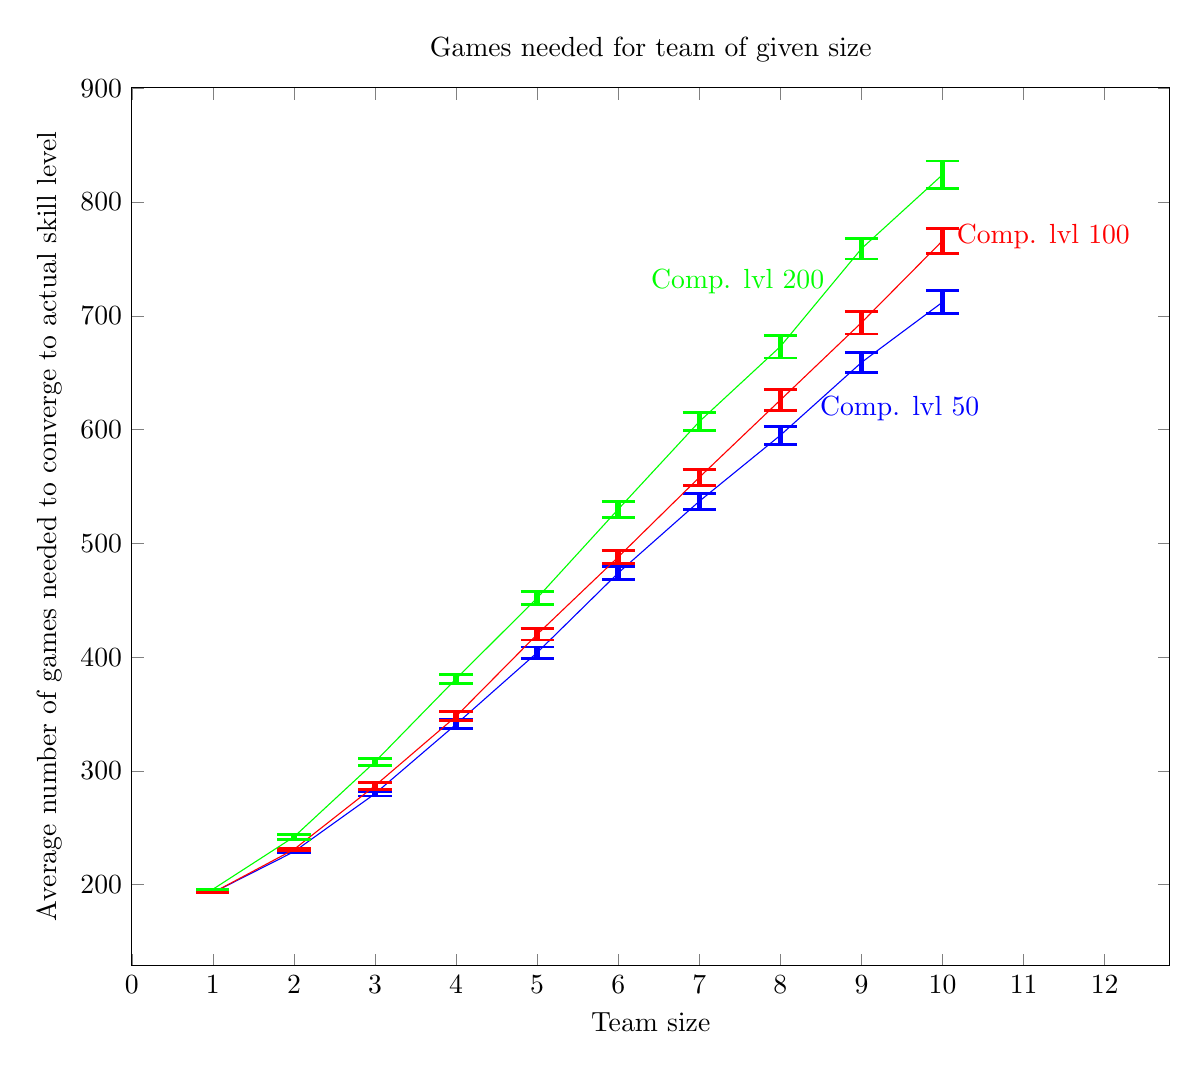
\begin{tikzpicture}
\begin{axis}[xmin=0,xmax=12.8,width = 420,xlabel=Team size,ylabel=Average number of games needed to converge to actual skill level,title=Games needed for team of given size]
\addplot[label=hoi,blue, error bars/.cd, y dir=both, y explicit, error bar style={line width=2pt}, error mark options={rotate=90,blue,mark size=6pt, line width=1pt}] plot coordinates {(1,193) +- (0,0) (2,229) +- (0,1) (3,280) +- (0,2) (4,341) +- (0,4) (5,404) +- (0,5) (6,474) +- (0,6) (7,537) +- (0,7) (8,595) +- (0,8) (9,659) +- (0,9) (10,712) +- (0,10)} node[right,pos=0.82] {Comp. lvl 50};
\addplot[red, error bars/.cd, y dir=both, y explicit, error bar style={line width=2pt}, error mark options={rotate=90,red,mark size=6pt, line width=1pt}] plot coordinates {(1,193) +- (0,0) (2,231) +- (0,1) (3,287) +- (0,3) (4,348) +- (0,4) (5,420) +- (0,5) (6,488) +- (0,6) (7,558) +- (0,7) (8,626) +- (0,9) (9,694) +- (0,10) (10,766) +- (0,11)} node[right,pos=1.007] {Comp. lvl 100};
\addplot[green, error bars/.cd, y dir=both, y explicit, error bar style={line width=2pt}, error mark options={rotate=90,green,mark size=6pt, line width=1pt}] plot coordinates {(1,196) +- (0,0) (2,242) +- (0,2) (3,308) +- (0,3) (4,381) +- (0,4) (5,452) +- (0,6) (6,530) +- (0,7) (7,607) +- (0,8) (8,673) +- (0,10) (9,759) +- (0,9) (10,824) +- (0,12)} node[left,pos=0.85] {Comp. lvl 200};
\end{axis}
\end{tikzpicture}
\begin{center}
\begin{minipage}{.8\textwidth}
\textbf{Figure 1:} Games needed for team of given size for competence ranges 50, 100 and 200.\\\\
\end{minipage}
\end{center}

\begin{tikzpicture}
\begin{axis}[width=420, xlabel=Number of games played ($x$),ylabel=Elo rating ($y$)]
\addplot[blue] table {player.dat} node[right,pos=0.4] {Player's Elo rating after playing $x$ games};
\addplot[red, samples = 100, domain=0:200]{2293} node[below,pos=0.3] {Player's true skill level};
\end{axis}
\end{tikzpicture}
\begin{center}
\begin{minipage}{.8\textwidth}
\textbf{Figure 2:} An example of the progress of the Elo rating of a player after playing $x$ games. Team sizes were $1$ in this case. The player has a true skill level of 2293.\\
\end{minipage}
\end{center}

\section{Discussion}
The figures show that there is a linear relation between the amount of games that are needed to converge a player's Elo rating towards their real skill level. The confidence intervals are small, while the average number of games can become high numbers for bigger teams. 

Compared to TrueSkill\texttrademark, the proposed program needs more games to converge a player's Elo to their true skill level. However, while TrueSkill\texttrademark is based on some of the fundamentals of Elo, it uses a Bayesian rating system.\cite{trueskill} For a game with 2 teams of 4 players each, TrueSkill\texttrademark needs approximately 46 games\cite{trueskillconvergence}, whereas the proposed system Elo system needs roughly 350 games, which is around 8 times as much. If a team consists of 8 players, TrueSkill\texttrademark needs 96 games, while the proposed program indicates that 595 games are needed to converge.\\
While TrueSkill\texttrademark does not particularly take the team sizes into account, the same positive linear relation can be found here. It can be noted that the program used in this paper will not be of any use in the real (gaming) world, because it does not show any advantages over TrueSkill\texttrademark.


\begin{quote}
	``However, there is another factor taken into consideration which is MVP (Most Valuable Player). MVP is given to a player which has done the most work for their team. Please note that a player with 5 kill can still lose the MVP to a person who defuses or successfully detonated the bomb. The reason for this is because, CSGO is a team-based game, a player can kill the whole enemy team but still lose the round because he may not have the defuser to defuse the bomb in time.''\cite{csgo}
\end{quote}

The program does not take into account anything specific about the current game, like MVP awards or the main weapon of choice of the player, which will increase a player's skill for that game and might get a higher win percentage for the current game. Last, the program does not take into account something like a draw, which suggests a good match\cite{trueskillconvergence}. Further research is needed to show if the mentioned factors like MVP and draws do really affect a player's convergence rate in relation to the size of the team.

\section{Conclusion}

The hypothesis posed in this paper stated that the size of a team in a particular game would influence the time it takes a player's rating to converge to the correct number. The results show that a positive linear relation can be found between team size and convergence time. This leads to the conclusion that the answer is yes; the size of a team impacts the overall convergence of the respective player's rating.
However, this does not yet answer the question posed at the start of this paper: Is gamer frustration justified? To justify the frustration expressed by gamers, one needs to prove that at some point there is nothing a player can do to climb to their allegedly higher rating.
For this to be true, an example is required where it takes excessively long for a player to climb to their own level. In contrast, though there have been examples in the simulations that did take long, it never occurred that the rating did not converge. Consequently, a sound conclusion would be that when a player is not able to climb for a long time, they have converged to their skill level and failure to climb further is to be blamed on themselves and themselves alone.


















% Your references go at the end of the main text, and before the
% figures.  For this document we've used BibTeX, the .bib file
% scibib.bib, and the .bst file Science.bst.  The package scicite.sty
% was included to format the reference numbers according to *Science*
% style.


\bibliography{scibib}

\bibliographystyle{Science}



% Following is a new environment, {scilastnote}, that's defined in the
% preamble and that allows authors to add a reference at the end of the
% list that's not signaled in the text; such references are used in
% *Science* for acknowledgments of funding, help, etc.





% For your review copy (i.e., the file you initially send in for
% evaluation), you can use the {figure} environment and the
% \includegraphics command to stream your figures into the text, placing
% all figures at the end.  For the final, revised manuscript for
% acceptance and production, however, PostScript or other graphics
% should not be streamed into your compliled file.  Instead, set
% captions as simple paragraphs (with a \noindent tag), setting them
% off from the rest of the text with a \clearpage as shown  below, and
% submit figures as separate files according to the Art Department's
% instructions.


\end{document}




















